\documentclass[border=6pt,tikz]{standalone}
\usepackage{amsmath,amssymb}
\usepackage{tikz}
\usetikzlibrary{arrows.meta,calc,decorations.pathreplacing,patterns,shapes.geometric,positioning,shadings,plotmarks}

\begin{document}
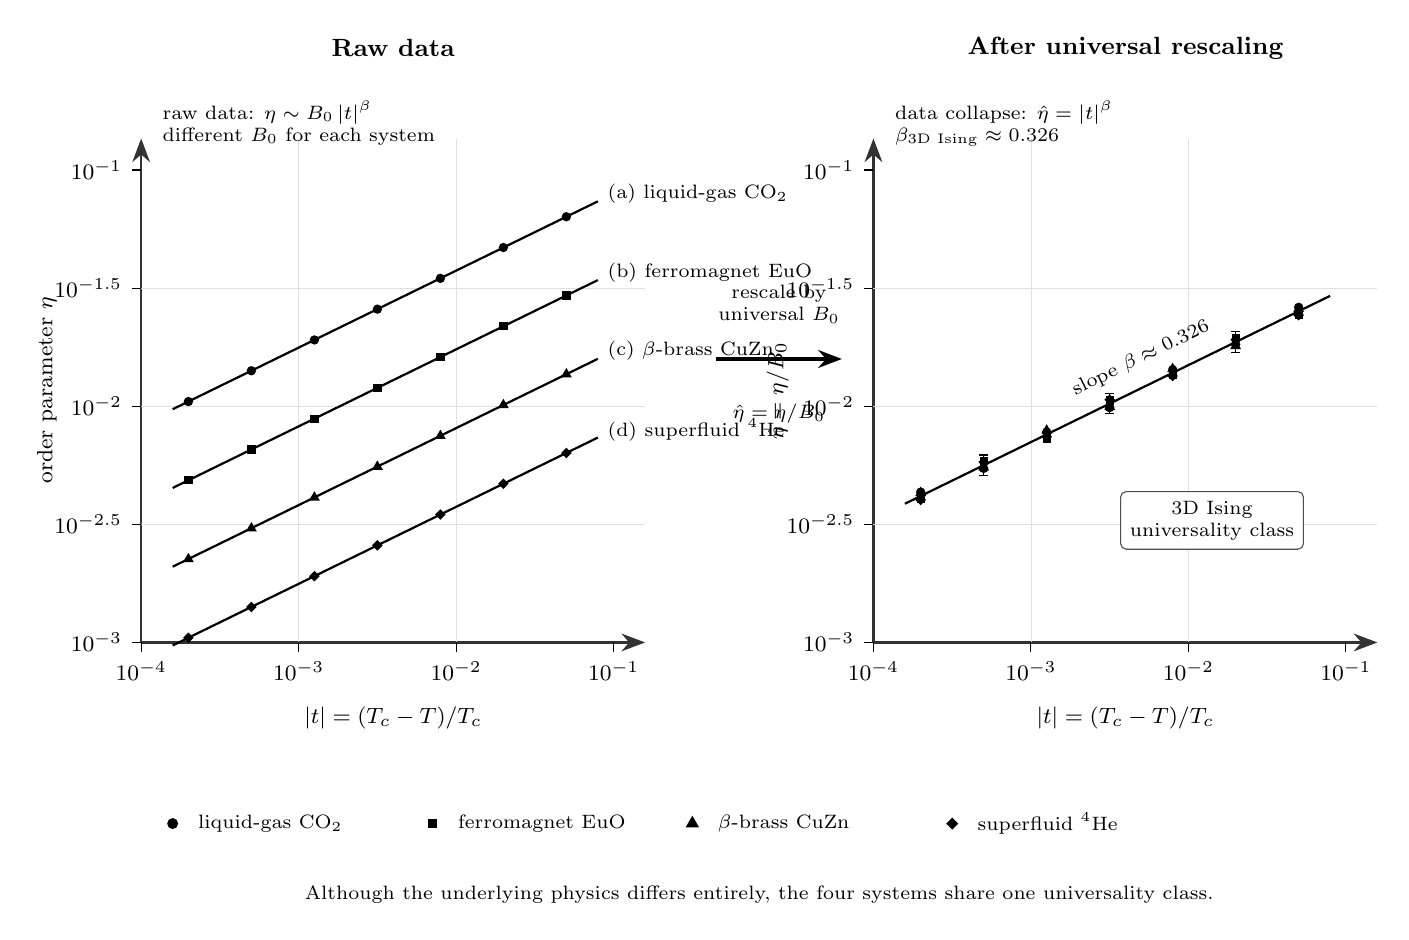
\begin{tikzpicture}[
  >={Stealth[length=3mm]},
  font=\small,
  axislabel/.style={font=\footnotesize},
  axisline/.style={->,thick,black!80},
  gridline/.style={very thin,gray!25},
  datapt/.style={draw=black!80,fill=black!10,thin},
  bandlabel/.style={font=\scriptsize}
]

%==============================================================
% LEFT PANEL: raw data, four parallel power-law bands
%   x-axis: log10|t| from -4 to -1  -> mapped to 0..6 cm  (1 cm per decade -> 3 decades; we use 6cm/3 decades = 2cm per decade)
%   y-axis: log10 eta arbitrary range  -> mapped to 0..6 cm
%   slope = beta ~= 0.326
%==============================================================
\begin{scope}[shift={(0,0)}]
  % box
  \draw[axisline] (0,0) -- (6.4,0);   % x axis
  \draw[axisline] (0,0) -- (0,6.4);   % y axis

  % x ticks at log10|t| = -4,-3,-2,-1   --> u = 0,2,4,6
  \foreach \k/\u/\lab in {-4/0/{$10^{-4}$},-3/2/{$10^{-3}$},-2/4/{$10^{-2}$},-1/6/{$10^{-1}$}}{
    \draw (\u,0) -- (\u,-0.12);
    \node[axislabel,below] at (\u,-0.12) {\lab};
  }
  % y ticks
  \foreach \v/\lab in {0/{$10^{-3}$},1.5/{$10^{-2.5}$},3/{$10^{-2}$},4.5/{$10^{-1.5}$},6/{$10^{-1}$}}{
    \draw (0,\v) -- (-0.12,\v);
    \node[axislabel,left] at (-0.12,\v) {\lab};
  }

  % grid (decades only)
  \foreach \u in {2,4}{ \draw[gridline] (\u,0) -- (\u,6.4); }
  \foreach \v in {1.5,3,4.5}{ \draw[gridline] (0,\v) -- (6.4,\v); }

  % axis titles
  \node[axislabel,below] at (3.2,-0.7) {$|t|=(T_c-T)/T_c$};
  \node[axislabel,rotate=90,above] at (-0.95,3.2) {order parameter $\eta$};

  % power-law bands: eta = B0 * |t|^beta. With slope beta in log-log,
  % using 2 cm = 1 decade in x, 1.5 cm = 0.5 decade in y, our drawn slope must be:
  % d(y_cm)/d(x_cm) = (3 cm/decade) * beta / (2 cm/decade) = 1.5*beta = 0.489
  % For beta=0.326: slope_cm = 0.489.
  % We pick four lines with intercept offsets DeltaY (in cm) at x=6 (top of |t|).
  % Line passes through (x_cm=6, y_cm = y6) with slope 0.489.
  % choose y6 values for the four systems
  % (a) liquid-gas CO2  : y6 = 5.7
  % (b) ferromagnet EuO : y6 = 4.7
  % (c) beta-brass CuZn : y6 = 3.7
  % (d) superfluid 4He  : y6 = 2.7

  % helper: line from (xL, yL) to (xR, yR) with slope 0.489
  % yL = y6 - 0.489 * (6 - 0) = y6 - 2.934
  % We draw from x=0.4 to x=5.8 to keep within axes
  % yL_draw = y6 - 0.489 * (6 - 0.4) = y6 - 2.738
  % yR_draw = y6 - 0.489 * (6 - 5.8) = y6 - 0.098

  % (a) CO2 - circles
  \draw[thick,black] (0.4, 2.962) -- (5.8, 5.602);
  \foreach \x in {0.6,1.4,2.2,3.0,3.8,4.6,5.4}{
    \pgfmathsetmacro{\y}{5.7 - 0.489*(6-\x)}
    \node[circle,fill=black,inner sep=1.2pt] at (\x,\y) {};
  }
  \node[bandlabel,right,black] at (5.8,5.7) {(a) liquid-gas CO$_2$};

  % (b) EuO - squares
  \draw[thick,black] (0.4, 1.962) -- (5.8, 4.602);
  \foreach \x in {0.6,1.4,2.2,3.0,3.8,4.6,5.4}{
    \pgfmathsetmacro{\y}{4.7 - 0.489*(6-\x)}
    \node[rectangle,fill=black,inner sep=1.2pt,minimum size=3pt] at (\x,\y) {};
  }
  \node[bandlabel,right,black] at (5.8,4.7) {(b) ferromagnet EuO};

  % (c) beta-brass - triangles
  \draw[thick,black] (0.4, 0.962) -- (5.8, 3.602);
  \foreach \x in {0.6,1.4,2.2,3.0,3.8,4.6,5.4}{
    \pgfmathsetmacro{\y}{3.7 - 0.489*(6-\x)}
    \node[regular polygon,regular polygon sides=3,fill=black,inner sep=0.8pt,minimum size=4pt] at (\x,\y) {};
  }
  \node[bandlabel,right,black] at (5.8,3.7) {(c) $\beta$-brass CuZn};

  % (d) superfluid 4He - diamonds
  \draw[thick,black] (0.4, -0.038) -- (5.8, 2.602);
  \foreach \x in {0.6,1.4,2.2,3.0,3.8,4.6,5.4}{
    \pgfmathsetmacro{\y}{2.7 - 0.489*(6-\x)}
    \node[diamond,fill=black,inner sep=0.6pt,minimum size=4pt] at (\x,\y) {};
  }
  \node[bandlabel,right,black] at (5.8,2.7) {(d) superfluid $^4$He};

  % side annotation
  \node[align=left,font=\scriptsize,anchor=north west] at (0.15,7.0)
    {raw data: $\eta\sim B_{0}\,|t|^{\beta}$\\different $B_{0}$ for each system};

  % panel title
  \node[font=\small\bfseries] at (3.2,7.55) {Raw data};

\end{scope}

%==============================================================
% Big arrow between panels: "rescale by universal B0"
%==============================================================
\begin{scope}[shift={(7.3,0)}]
  \draw[->,line width=1.4pt,black] (0,3.6) -- (1.6,3.6);
  \node[align=center,font=\scriptsize] at (0.8,4.3) {rescale by\\universal $B_{0}$};
  \node[align=center,font=\scriptsize] at (0.8,2.9) {$\hat\eta=\eta/B_{0}$};
\end{scope}

%==============================================================
% RIGHT PANEL: collapsed data, all on a single universal line
%==============================================================
\begin{scope}[shift={(9.3,0)}]
  \draw[axisline] (0,0) -- (6.4,0);
  \draw[axisline] (0,0) -- (0,6.4);

  % x ticks
  \foreach \k/\u/\lab in {-4/0/{$10^{-4}$},-3/2/{$10^{-3}$},-2/4/{$10^{-2}$},-1/6/{$10^{-1}$}}{
    \draw (\u,0) -- (\u,-0.12);
    \node[axislabel,below] at (\u,-0.12) {\lab};
  }
  \foreach \v/\lab in {0/{$10^{-3}$},1.5/{$10^{-2.5}$},3/{$10^{-2}$},4.5/{$10^{-1.5}$},6/{$10^{-1}$}}{
    \draw (0,\v) -- (-0.12,\v);
    \node[axislabel,left] at (-0.12,\v) {\lab};
  }
  \foreach \u in {2,4}{ \draw[gridline] (\u,0) -- (\u,6.4); }
  \foreach \v in {1.5,3,4.5}{ \draw[gridline] (0,\v) -- (6.4,\v); }

  \node[axislabel,below] at (3.2,-0.7) {$|t|=(T_c-T)/T_c$};
  \node[axislabel,rotate=90,above] at (-0.95,3.2) {$\hat\eta=\eta/B_{0}$};

  % single universal line; choose y6 = 4.5 for visibility
  % yL = 4.5 - 0.489*(6-0.4) = 4.5 - 2.738 = 1.762
  % yR = 4.5 - 0.489*(6-5.8) = 4.5 - 0.098 = 4.402
  \draw[thick,black] (0.4,1.762) -- (5.8,4.402);

  % overlapping symbols at the same x positions, with tiny vertical jitter ~ +-0.05cm
  \foreach \x/\j in {0.6/0.05,1.4/-0.04,2.2/0.03,3.0/-0.05,3.8/0.04,4.6/-0.03,5.4/0.05}{
    \pgfmathsetmacro{\yc}{4.5 - 0.489*(6-\x) + \j}
    \node[circle,fill=black,inner sep=1.2pt] at (\x,\yc) {};
  }
  \foreach \x/\j in {0.6/-0.04,1.4/0.05,2.2/-0.05,3.0/0.04,3.8/-0.03,4.6/0.05,5.4/-0.04}{
    \pgfmathsetmacro{\yc}{4.5 - 0.489*(6-\x) + \j}
    \node[rectangle,fill=black,inner sep=1.2pt,minimum size=3pt] at (\x,\yc) {};
  }
  \foreach \x/\j in {0.6/0.04,1.4/-0.03,2.2/0.05,3.0/-0.04,3.8/0.05,4.6/-0.05,5.4/0.03}{
    \pgfmathsetmacro{\yc}{4.5 - 0.489*(6-\x) + \j}
    \node[regular polygon,regular polygon sides=3,fill=black,inner sep=0.8pt,minimum size=4pt] at (\x,\yc) {};
  }
  \foreach \x/\j in {0.6/-0.05,1.4/0.04,2.2/-0.03,3.0/0.05,3.8/-0.04,4.6/0.03,5.4/-0.05}{
    \pgfmathsetmacro{\yc}{4.5 - 0.489*(6-\x) + \j}
    \node[diamond,fill=black,inner sep=0.6pt,minimum size=4pt] at (\x,\yc) {};
  }

  % error bars at three points (vertical +- 3% of value -> in log space tiny)
  \foreach \x in {1.4,3.0,4.6}{
    \pgfmathsetmacro{\yc}{4.5 - 0.489*(6-\x)}
    \draw[thin,black] (\x,\yc-0.13) -- (\x,\yc+0.13);
    \draw[thin,black] (\x-0.06,\yc-0.13) -- (\x+0.06,\yc-0.13);
    \draw[thin,black] (\x-0.06,\yc+0.13) -- (\x+0.06,\yc+0.13);
  }

  % slope label along the line
  \node[font=\scriptsize,rotate=26,above,black] at (3.5,3.4) {slope $\beta\approx 0.326$};

  % universality class label, central
  \node[draw=black!70,fill=white,rounded corners=2pt,font=\scriptsize,align=center] at (4.3,1.55)
    {3D Ising\\universality class};

  % side annotation
  \node[align=left,font=\scriptsize,anchor=north west] at (0.15,7.0)
    {data collapse: $\hat\eta=|t|^{\beta}$\\$\beta_{\text{3D Ising}}\approx 0.326$};

  % panel title
  \node[font=\small\bfseries] at (3.2,7.55) {After universal rescaling};
\end{scope}

%==============================================================
% Legend strip (symbol key) below both panels
%==============================================================
\begin{scope}[shift={(0,-2.3)}]
  \node[circle,fill=black,inner sep=1.4pt] at (0.4,0) {};
  \node[anchor=west,font=\scriptsize] at (0.6,0) {liquid-gas CO$_2$};

  \node[rectangle,fill=black,inner sep=1.4pt,minimum size=3.5pt] at (3.7,0) {};
  \node[anchor=west,font=\scriptsize] at (3.9,0) {ferromagnet EuO};

  \node[regular polygon,regular polygon sides=3,fill=black,inner sep=1pt,minimum size=4pt] at (7.0,0) {};
  \node[anchor=west,font=\scriptsize] at (7.2,0) {$\beta$-brass CuZn};

  \node[diamond,fill=black,inner sep=0.7pt,minimum size=4.5pt] at (10.3,0) {};
  \node[anchor=west,font=\scriptsize] at (10.5,0) {superfluid $^4$He};
\end{scope}

%==============================================================
% Bottom note
%==============================================================
\node[align=center,font=\scriptsize] at (7.85,-3.2)
  {Although the underlying physics differs entirely, the four systems share one universality class.};

\end{tikzpicture}
\end{document}
